\documentclass[a4paper,11pt]{article}
\usepackage[margin=2cm]{geometry}
\usepackage{amsmath,amssymb,amsthm}
\usepackage{tikz}
\usepackage[dvipsnames]{xcolor}
\usetikzlibrary{arrows.meta,positioning,calc}

\tikzset{
    triple/.style={circle, draw, inner sep=2pt, minimum size=18pt, font=\scriptsize},
    fp/.style={triple, fill=yellow!40},
    matched/.style={triple, fill=green!20},
    balanced/.style={triple, fill=red!20, dashed},
    posobj/.style={rectangle, draw=blue!70, fill=blue!10, rounded corners=2pt,
                   inner sep=3pt, font=\scriptsize},
    negobj/.style={rectangle, draw=red!70, fill=red!10, rounded corners=2pt,
                   inner sep=3pt, font=\scriptsize},
    fpobj/.style={rectangle, draw=OliveGreen!70, fill=green!10, rounded corners=2pt,
                  inner sep=3pt, font=\scriptsize},
    pairline/.style={<->, thick, gray!60},
    injline/.style={->, thick, blue!60},
}

\newcommand{\qbin}[2]{\genfrac{[}{]}{0pt}{}{#1}{#2}}

\begin{document}

% ============================================================
% FIGURE 1: The Slack Simplex and Injection (d=4)
% ============================================================
\begin{center}
\textbf{\large Figure 1: Injection objects --- max-1 CPP triples on the slack simplex}\\[4pt]
\textit{Profile $c = (2,1,1)$, $d = 4$. Slack $s = (s_1, s_2, s_3)$, $s_1{+}s_2{+}s_3 = 4$.}
\end{center}

\bigskip

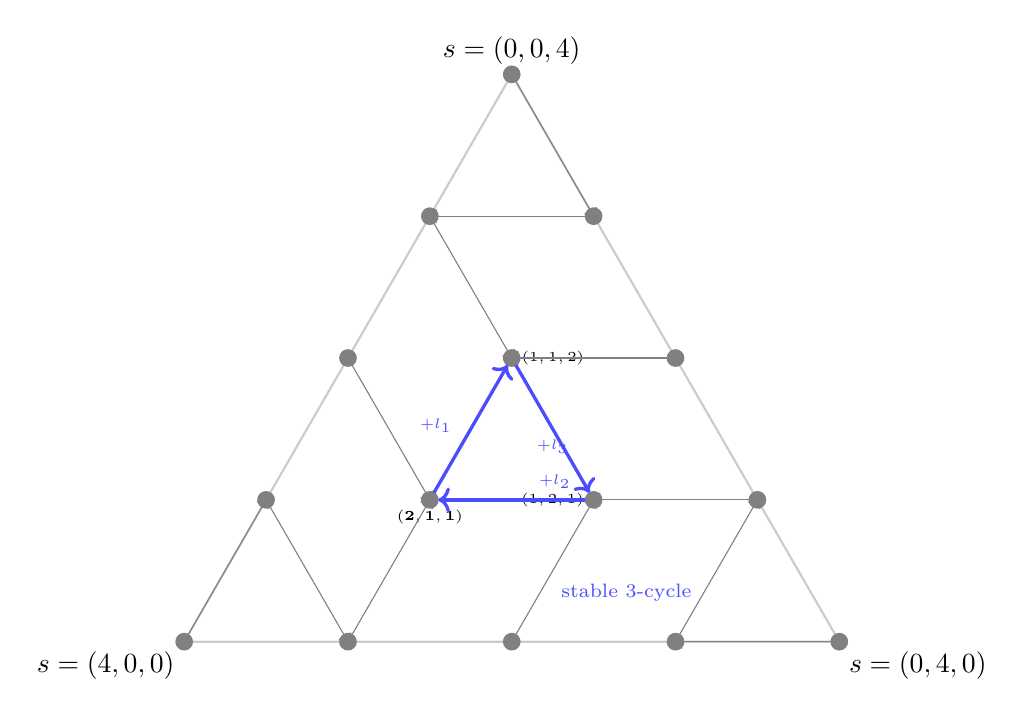
\begin{tikzpicture}[scale=1.6]
  % Draw the simplex (equilateral triangle)
  % Barycentric coords: (s1,s2,s3) with s1+s2+s3=4
  % Map to Cartesian: x = s2 + s3/2, y = s3 * sqrt(3)/2
  % Scaled so the triangle has side length ~6

  \def\sc{1.3}  % scale factor
  \def\bary#1#2#3{({(\sc)*(#2 + #3/2)}, {(\sc)*(#3*0.866)})}

  % Triangle outline
  \draw[gray!40, thick]
    \bary{4}{0}{0} -- \bary{0}{4}{0} -- \bary{0}{0}{4} -- cycle;

  % Vertex labels
  \node[below left] at \bary{4}{0}{0} {$s=(4,0,0)$};
  \node[below right] at \bary{0}{4}{0} {$s=(0,4,0)$};
  \node[above] at \bary{0}{0}{4} {$s=(0,0,4)$};

  % All 15 lattice points with injection arrows
  % Each point labeled by slack, arrow shows which component is incremented

  % Interior and boundary points
  % The injection rule: at each slack, the arrow shows phi direction
  % (s_k decreases by 1, s_{k-2 mod 3} increases by 1)

  % Draw all lattice points
  \foreach \a/\b/\c in {
    4/0/0, 3/1/0, 3/0/1, 2/2/0, 2/1/1, 2/0/2,
    1/3/0, 1/2/1, 1/1/2, 1/0/3,
    0/4/0, 0/3/1, 0/2/2, 0/1/3, 0/0/4} {
    \fill[black!50] \bary{\a}{\b}{\c} circle (2pt);
  }

  % Label some key slacks
  \node[font=\tiny, below] at \bary{2}{1}{1} {$\mathbf{(2,1,1)}$};
  \node[font=\tiny, right] at \bary{1}{1}{2} {$(1,1,2)$};
  \node[font=\tiny, left] at \bary{1}{2}{1} {$(1,2,1)$};

  % Draw the absorbing cycle (the "stable orbit")
  % Slightly offset the arrows so they don't overlap the nodes
  \draw[very thick, blue!70, ->, shorten >=3pt, shorten <=3pt]
    \bary{2}{1}{1} -- node[font=\tiny,above left,pos=0.4]{$+l_1$} \bary{1}{1}{2};
  \draw[very thick, blue!70, ->, shorten >=3pt, shorten <=3pt]
    \bary{1}{1}{2} -- node[font=\tiny,below,pos=0.5]{$+l_3$} \bary{1}{2}{1};
  \draw[very thick, blue!70, ->, shorten >=3pt, shorten <=3pt]
    \bary{1}{2}{1} -- node[font=\tiny,above right,pos=0.4]{$+l_2$} \bary{2}{1}{1};

  % Mark the cycle
  \node[font=\scriptsize, blue!70] at ($({\sc*2.7},{\sc*0.3})$)
    {stable 3-cycle};

  % Draw injection arrows from other slacks into the cycle
  \draw[thin, gray, ->] \bary{4}{0}{0} -- \bary{3}{0}{1};
  \draw[thin, gray, ->] \bary{3}{1}{0} -- \bary{2}{1}{1};
  \draw[thin, gray, ->] \bary{3}{0}{1} -- \bary{3}{1}{0};
  \draw[thin, gray, ->] \bary{2}{2}{0} -- \bary{1}{2}{1};
  \draw[thin, gray, ->] \bary{2}{0}{2} -- \bary{2}{1}{1};
  \draw[thin, gray, ->] \bary{1}{3}{0} -- \bary{0}{3}{1};
  \draw[thin, gray, ->] \bary{1}{0}{3} -- \bary{1}{1}{2};
  \draw[thin, gray, ->] \bary{0}{4}{0} -- \bary{1}{3}{0};
  \draw[thin, gray, ->] \bary{0}{3}{1} -- \bary{1}{2}{1};
  \draw[thin, gray, ->] \bary{0}{2}{2} -- \bary{1}{1}{2};
  \draw[thin, gray, ->] \bary{0}{1}{3} -- \bary{1}{0}{3};
  \draw[thin, gray, ->] \bary{0}{0}{4} -- \bary{0}{1}{3};

\end{tikzpicture}

\bigskip

% ============================================================
% FIGURE 2: Weight-by-weight injection (d=4)
% ============================================================
\begin{center}
\textbf{\large Figure 2: The injection $\phi$ weight by weight}\\[4pt]
\textit{$c=(2,1,1)$. Each triple $(l_1,l_2,l_3)$ shown with its slack.
Yellow = fixed point (not in image of $\phi$).}
\end{center}

\bigskip

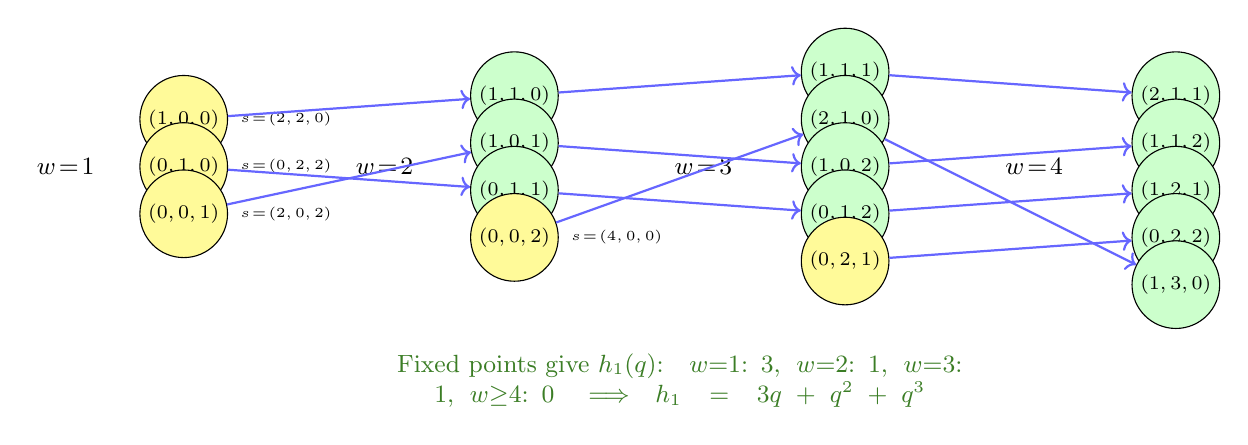
\begin{tikzpicture}[xscale=3.0, yscale=0.75]
  % Weight 1 (3 triples, all FPs since no predecessors)
  \node[font=\small\bfseries] at (-0.5, 0) {$w\!=\!1$};
  \node[fp] (w1a) at (0, 0.8)  {$(1,0,0)$};
  \node[fp] (w1b) at (0, 0)    {$(0,1,0)$};
  \node[fp] (w1c) at (0, -0.8) {$(0,0,1)$};
  \node[font=\tiny, right=1pt] at (w1a.east) {$s\!=\!(2,2,0)$};
  \node[font=\tiny, right=1pt] at (w1b.east) {$s\!=\!(0,2,2)$};
  \node[font=\tiny, right=1pt] at (w1c.east) {$s\!=\!(2,0,2)$};

  % Weight 2 (4 triples, 3 matched + 1 FP)
  \node[font=\small\bfseries] at (0.85, 0) {$w\!=\!2$};
  \node[matched] (w2a) at (1.4, 1.2) {$(1,1,0)$};
  \node[matched] (w2b) at (1.4, 0.4) {$(1,0,1)$};
  \node[matched] (w2c) at (1.4, -0.4) {$(0,1,1)$};
  \node[fp]      (w2d) at (1.4, -1.2) {$(0,0,2)$};
  \node[font=\tiny, right=1pt] at (w2d.east) {$s\!=\!(4,0,0)$};

  \draw[injline] (w1a) -- (w2a);
  \draw[injline] (w1b) -- (w2c);
  \draw[injline] (w1c) -- (w2b);

  % Weight 3 (5 triples, 4 matched + 1 FP)
  \node[font=\small\bfseries] at (2.2, 0) {$w\!=\!3$};
  \node[matched] (w3a) at (2.8, 1.6) {$(1,1,1)$};
  \node[matched] (w3b) at (2.8, 0.8) {$(2,1,0)$};
  \node[matched] (w3c) at (2.8, 0)   {$(1,0,2)$};
  \node[matched] (w3d) at (2.8, -0.8){$(0,1,2)$};
  \node[fp]      (w3e) at (2.8, -1.6){$(0,2,1)$};

  \draw[injline] (w2a) -- (w3a);
  \draw[injline] (w2b) -- (w3c);
  \draw[injline] (w2c) -- (w3d);
  \draw[injline] (w2d) -- (w3b);

  % Weight 4 (5 triples, all matched from w=3, 0 FPs)
  \node[font=\small\bfseries] at (3.6, 0) {$w\!=\!4$};
  \node[matched] (w4a) at (4.2, 1.2) {$(2,1,1)$};
  \node[matched] (w4b) at (4.2, 0.4) {$(1,1,2)$};
  \node[matched] (w4c) at (4.2, -0.4){$(1,2,1)$};
  \node[matched] (w4d) at (4.2, -1.2){$(0,2,2)$};
  \node[matched] (w4e) at (4.2, -2.0){$(1,3,0)$};

  \draw[injline] (w3a) -- (w4a);
  \draw[injline] (w3b) -- (w4e);
  \draw[injline] (w3c) -- (w4b);
  \draw[injline] (w3d) -- (w4c);
  \draw[injline] (w3e) -- (w4d);

  % Annotation: h_1 from FPs (placed below the diagram)
  \node[font=\small, text=OliveGreen, anchor=north, text width=10cm, align=center]
    at (2.1, -3.0) {
    Fixed points give $h_1(q)$:\quad
    $w{=}1$: 3,\; $w{=}2$: 1,\; $w{=}3$: 1,\; $w{\geq}4$: 0
    \quad$\Longrightarrow$\quad $h_1 = 3q + q^2 + q^3$
  };

\end{tikzpicture}

\vspace{2cm}

% ============================================================
% FIGURE 3: A max-1 CPP as a triple of column partitions
% ============================================================
\begin{center}
\textbf{\large Figure 3: A max-1 CPP triple as column partitions}\\[4pt]
\textit{$c=(2,1,1)$, triple $(l_1,l_2,l_3) = (2,1,1)$, weight $w = 4$, slack $s = (2,1,1)$.}
\end{center}

\bigskip

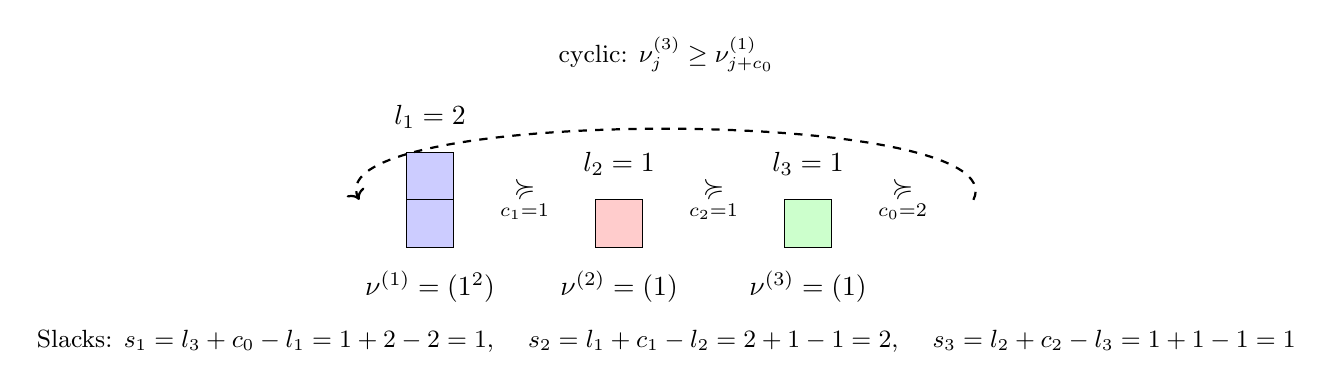
\begin{tikzpicture}[scale=0.6]
  % nu^1 = (1,1) (two parts of size 1, i.e., two rows of length 1)
  \begin{scope}[shift={(0,0)}]
    \draw[fill=blue!20] (0,0) rectangle (1,1);
    \draw[fill=blue!20] (0,1) rectangle (1,2);
    \draw (0,0) grid (1,2);
    \node[below] at (0.5, -0.3) {$\nu^{(1)} = (1^2)$};
    \node[above] at (0.5, 2.3) {$l_1 = 2$};
  \end{scope}

  % Interlacing arrow
  \node at (2.5, 1) {$\underset{c_1=1}{\succcurlyeq}$};

  % nu^2 = (1) (one part of size 1)
  \begin{scope}[shift={(4,0)}]
    \draw[fill=red!20] (0,0) rectangle (1,1);
    \draw (0,0) grid (1,1);
    \node[below] at (0.5, -0.3) {$\nu^{(2)} = (1)$};
    \node[above] at (0.5, 1.3) {$l_2 = 1$};
  \end{scope}

  % Interlacing arrow
  \node at (6.5, 1) {$\underset{c_2=1}{\succcurlyeq}$};

  % nu^3 = (1) (one part of size 1)
  \begin{scope}[shift={(8,0)}]
    \draw[fill=green!20] (0,0) rectangle (1,1);
    \draw (0,0) grid (1,1);
    \node[below] at (0.5, -0.3) {$\nu^{(3)} = (1)$};
    \node[above] at (0.5, 1.3) {$l_3 = 1$};
  \end{scope}

  % Interlacing arrow (cyclic)
  \node at (10.5, 1) {$\underset{c_0=2}{\succcurlyeq}$};

  % Wrap-around indicator
  \draw[dashed, thick, ->] (12, 1) .. controls (13, 3) and (-2, 3) .. (-1, 1);
  \node[above] at (5.5, 3.5) {\small cyclic: $\nu^{(3)}_j \geq \nu^{(1)}_{j+c_0}$};

  % Slack annotation
  \node[font=\small] at (5.5, -2) {
    Slacks: $s_1 = l_3 + c_0 - l_1 = 1+2-2 = 1$, \quad
    $s_2 = l_1 + c_1 - l_2 = 2+1-1 = 2$, \quad
    $s_3 = l_2 + c_2 - l_3 = 1+1-1 = 1$
  };
\end{tikzpicture}

\newpage

% ============================================================
% FIGURE 4: Involution objects for n=1
% ============================================================
\begin{center}
\textbf{\large Figure 4: Signed objects for the involution ($n=1$, $c=(2,1,1)$)}\\[4pt]
\textit{$Q_1 = h_1 - q \cdot h_0 = (3q + q^2 + q^3) - q = 2q + q^2 + q^3$}
\end{center}

\bigskip

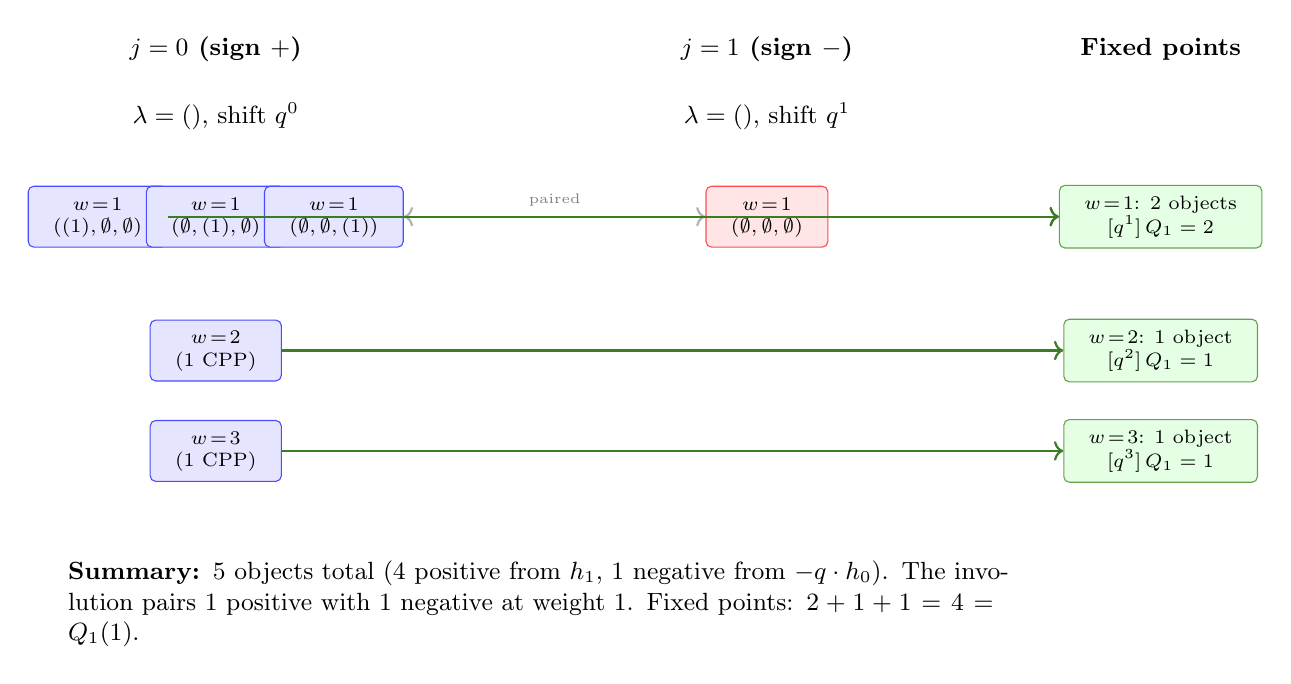
\begin{tikzpicture}[xscale=1.0, yscale=0.85]
  % Column headers
  \node[font=\small\bfseries] at (0, 6) {$j=0$ (sign $+$)};
  \node[font=\small\bfseries] at (7, 6) {$j=1$ (sign $-$)};
  \node[font=\small\bfseries] at (12, 6) {Fixed points};

  % j=0 term: h_1 objects, lambda=(), sign = +
  % h_1 = 3q + q^2 + q^3
  % Weight = 0 + 0 + w_h = w_h (T_0 = 0, |lambda| = 0)

  \node[font=\small] at (0, 5) {$\lambda = ()$, shift $q^0$};

  % Weight 1: 3 CPPs
  \node[posobj] (p1a) at (-1.5, 3.5)
    {\begin{tabular}{c}$w\!=\!1$\\ $((1),\emptyset,\emptyset)$\end{tabular}};
  \node[posobj] (p1b) at (0, 3.5)
    {\begin{tabular}{c}$w\!=\!1$\\ $(\emptyset,(1),\emptyset)$\end{tabular}};
  \node[posobj] (p1c) at (1.5, 3.5)
    {\begin{tabular}{c}$w\!=\!1$\\ $(\emptyset,\emptyset,(1))$\end{tabular}};

  % Weight 2: 1 CPP
  \node[posobj] (p2) at (0, 1.5)
    {\begin{tabular}{c}$w\!=\!2$\\$(1\text{ CPP})$\end{tabular}};

  % Weight 3: 1 CPP
  \node[posobj] (p3) at (0, 0)
    {\begin{tabular}{c}$w\!=\!3$\\$(1\text{ CPP})$\end{tabular}};

  % j=1 term: -q * h_0, lambda=(), sign = -
  % h_0 = 1. T_1 = 1. So single object at weight 1.
  \node[font=\small] at (7, 5) {$\lambda = ()$, shift $q^1$};

  \node[negobj] (n1) at (7, 3.5)
    {\begin{tabular}{c}$w\!=\!1$\\ $(\emptyset,\emptyset,\emptyset)$\end{tabular}};

  % Pairing
  \draw[pairline] (p1c) -- node[above, font=\tiny, gray]{paired} (n1);

  % Fixed points
  \node[fpobj] (f1a) at (12, 3.5)
    {\begin{tabular}{c}$w\!=\!1$: 2 objects\\ $[q^1]\,Q_1 = 2$\end{tabular}};
  \node[fpobj] (f2) at (12, 1.5)
    {\begin{tabular}{c}$w\!=\!2$: 1 object\\ $[q^2]\,Q_1 = 1$\end{tabular}};
  \node[fpobj] (f3) at (12, 0)
    {\begin{tabular}{c}$w\!=\!3$: 1 object\\ $[q^3]\,Q_1 = 1$\end{tabular}};

  \draw[->, OliveGreen, thick] (p1a) -- (f1a);
  \draw[->, OliveGreen, thick] (p1b) -- (f1a);
  \draw[->, OliveGreen, thick] (p2) -- (f2);
  \draw[->, OliveGreen, thick] (p3) -- (f3);

  % Summary
  \node[font=\small, text width=12cm, anchor=north west] at (-2, -1.5) {
    \textbf{Summary:} 5 objects total (4 positive from $h_1$, 1 negative from $-q \cdot h_0$).
    The involution pairs 1 positive with 1 negative at weight 1.
    Fixed points: $2 + 1 + 1 = 4 = Q_1(1)$.
  };
\end{tikzpicture}

\vspace{1.5cm}

% ============================================================
% FIGURE 5: Signed objects for n=2 (more complex)
% ============================================================
\begin{center}
\textbf{\large Figure 5: Signed objects for the involution ($n=2$, $c=(2,1,1)$)}\\[4pt]
\textit{$Q_2 = h_2 - q(1{+}q)\,h_1 + q^3 \cdot h_0$}
\end{center}

\bigskip

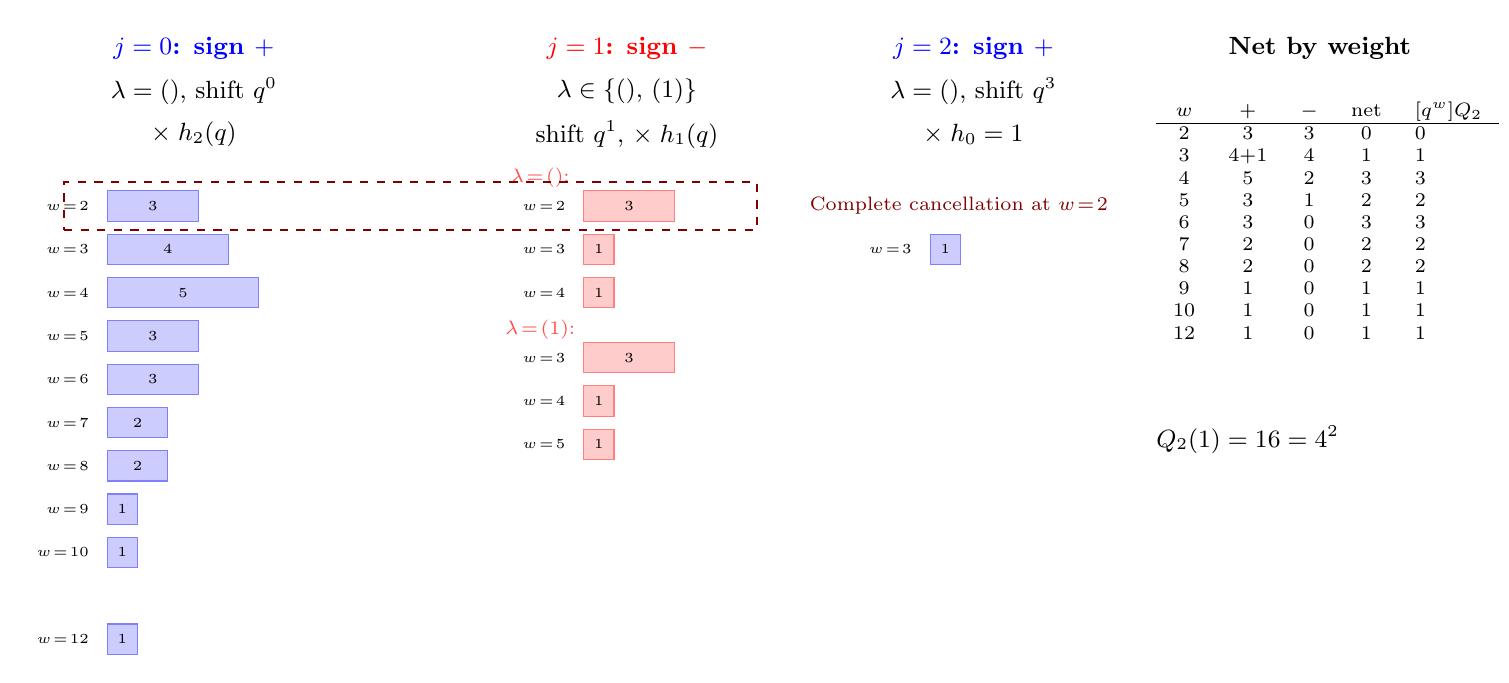
\begin{tikzpicture}[yscale=0.55, xscale=1.1]
  % Three j-terms as columns

  % j=0: sign +, h_2 objects
  \node[font=\small\bfseries, blue] at (0, 14) {$j=0$: sign $+$};
  \node[font=\small] at (0, 13) {$\lambda = ()$, shift $q^0$};
  \node[font=\small] at (0, 12) {$\times\; h_2(q)$};

  % Draw h_2 contribution bars
  \foreach \w/\cnt/\y in {
    2/3/10, 3/4/9, 4/5/8, 5/3/7, 6/3/6, 7/2/5, 8/2/4, 9/1/3, 10/1/2, 12/1/0} {
    \draw[fill=blue!20, draw=blue!50] (-1, \y) rectangle ({-1+\cnt*0.35}, {\y+0.7});
    \node[font=\tiny, left] at (-1.1, {\y+0.35}) {$w\!=\!\w$};
    \node[font=\tiny] at ({-1+\cnt*0.35/2}, {\y+0.35}) {\cnt};
  }

  % j=1: sign -, q*(1+q)*h_1
  \node[font=\small\bfseries, red] at (5, 14) {$j=1$: sign $-$};
  \node[font=\small] at (5, 13) {$\lambda \in \{(),\, (1)\}$};
  \node[font=\small] at (5, 12) {shift $q^1$, $\times\; h_1(q)$};

  % lambda=(): shift q, times h_1
  \node[font=\scriptsize, red!70] at (4, 11) {$\lambda\!=\!()$:};
  \foreach \w/\cnt/\y in {2/3/10, 3/1/9, 4/1/8} {
    \draw[fill=red!20, draw=red!50] (4.5, \y) rectangle ({4.5+\cnt*0.35}, {\y+0.7});
    \node[font=\tiny, left] at (4.4, {\y+0.35}) {$w\!=\!\w$};
    \node[font=\tiny] at ({4.5+\cnt*0.35/2}, {\y+0.35}) {\cnt};
  }

  % lambda=(1): shift q^2, times h_1
  \node[font=\scriptsize, red!70] at (4, 7.5) {$\lambda\!=\!(1)$:};
  \foreach \w/\cnt/\y in {3/3/6.5, 4/1/5.5, 5/1/4.5} {
    \draw[fill=red!20, draw=red!50] (4.5, \y) rectangle ({4.5+\cnt*0.35}, {\y+0.7});
    \node[font=\tiny, left] at (4.4, {\y+0.35}) {$w\!=\!\w$};
    \node[font=\tiny] at ({4.5+\cnt*0.35/2}, {\y+0.35}) {\cnt};
  }

  % j=2: sign +, q^3 * h_0
  \node[font=\small\bfseries, blue] at (9, 14) {$j=2$: sign $+$};
  \node[font=\small] at (9, 13) {$\lambda = ()$, shift $q^3$};
  \node[font=\small] at (9, 12) {$\times\; h_0 = 1$};

  \draw[fill=blue!20, draw=blue!50] (8.5, 9) rectangle (8.85, 9.7);
  \node[font=\tiny, left] at (8.4, 9.35) {$w\!=\!3$};
  \node[font=\tiny] at (8.675, 9.35) {1};

  % Summary table on the right
  \node[font=\small\bfseries] at (13, 14) {Net by weight};
  \node[font=\scriptsize, text width=4cm, anchor=north west] at (11, 13) {
    \begin{tabular}{ccccl}
    $w$ & $+$ & $-$ & net & $[q^w]Q_2$\\
    \hline
    2 & 3 & 3 & 0 & 0\\
    3 & 4+1 & 4 & 1 & 1\\
    4 & 5 & 2 & 3 & 3\\
    5 & 3 & 1 & 2 & 2\\
    6 & 3 & 0 & 3 & 3\\
    7 & 2 & 0 & 2 & 2\\
    8 & 2 & 0 & 2 & 2\\
    9 & 1 & 0 & 1 & 1\\
    10 & 1 & 0 & 1 & 1\\
    12 & 1 & 0 & 1 & 1\\
    \end{tabular}
  };

  \node[font=\small, anchor=north west] at (11, 5.5) {
    $Q_2(1) = 16 = 4^2$
  };

  % Annotation about complete cancellation at w=2
  \draw[thick, dashed, Maroon] (-1.5, 9.8) -- (6.5, 9.8) -- (6.5, 10.9) -- (-1.5, 10.9) -- cycle;
  \node[font=\scriptsize, Maroon, anchor=west] at (7, 10.35) {Complete cancellation at $w\!=\!2$};

\end{tikzpicture}

\vspace{1.5cm}

% ============================================================
% FIGURE 6: The finest decomposition (j, lambda, S, pi)
% ============================================================
\begin{center}
\textbf{\large Figure 6: Finest signed objects $(j, \lambda, S, \pi)$ for $n=1$, $c=(2,1,1)$}\\[4pt]
\textit{Expanding $(q)_1 = 1 - q$ gives subsets $S \subseteq \{1\}$.
Sign $= (-1)^{j+|S|}$.}
\end{center}

\bigskip

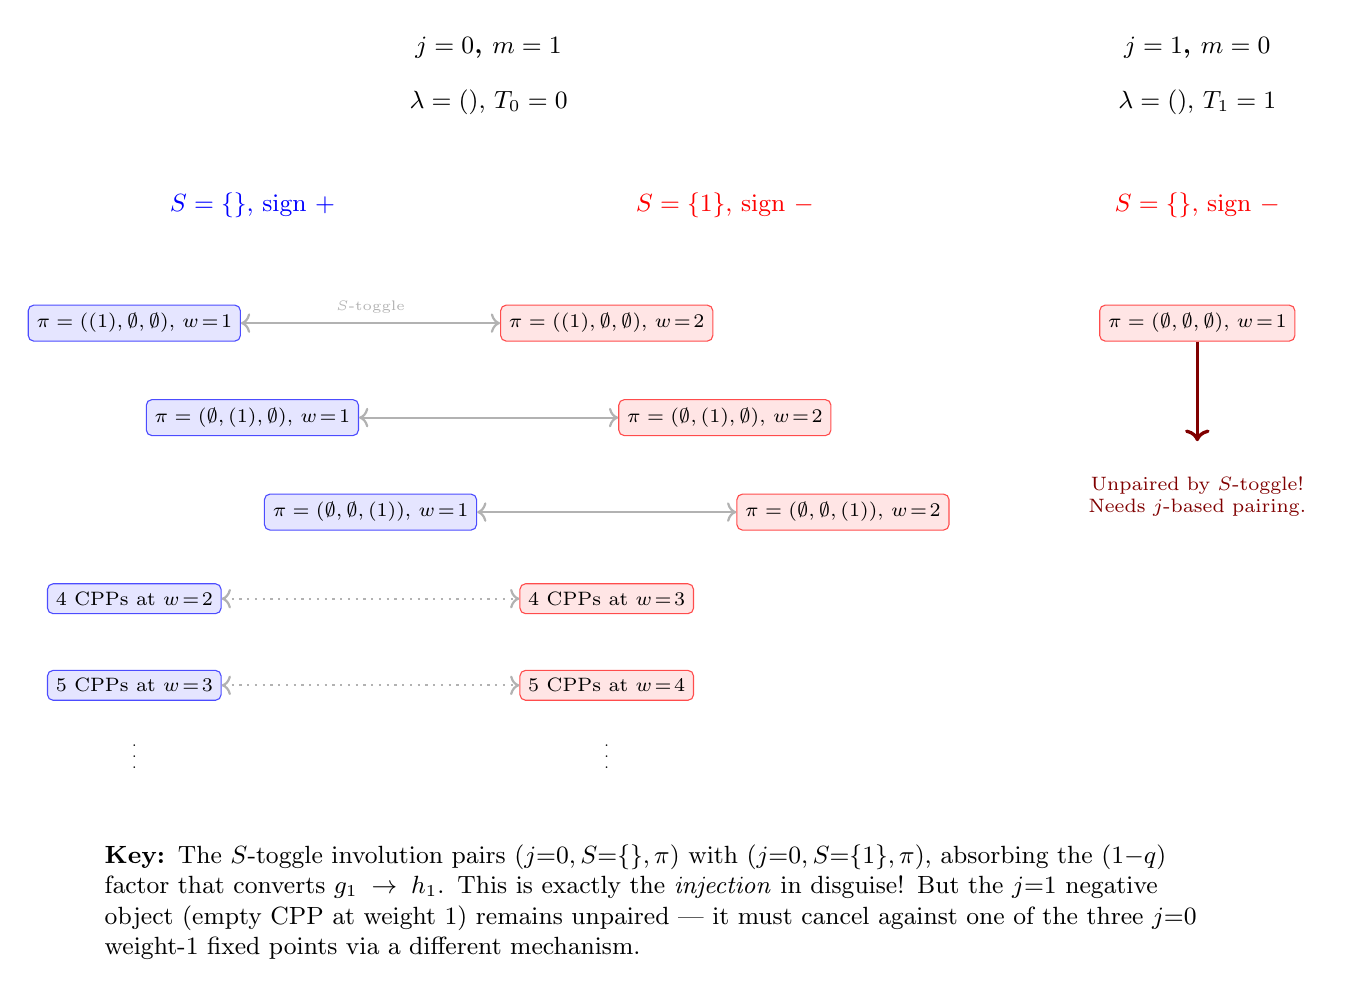
\begin{tikzpicture}[yscale=1.0, xscale=1.0]
  % Four groups: (j, S) determines sign
  % j=0, S={}: sign +   (the h_1 objects, i.e., (q)_1 * g_1 at S=empty)
  % j=0, S={1}: sign -  (the -(q)_1 * g_1 at S={1})
  % j=1, S={}: sign -   (the -q * (q)_0 * g_0 at S=empty)
  % j=1, S={1}: not possible since m=n-j=0, so S subset of {} only

  % Actually for n=1:
  % j=0, m=1: S in {{},{1}}, pi with max=1
  %   sign = (-1)^{0+|S|}
  % j=1, m=0: S in {{}}, pi = empty
  %   sign = (-1)^{1+0} = -1

  \node[font=\small\bfseries] at (0, 5.5) {$j=0$, $m=1$};
  \node[font=\small] at (0, 4.8) {$\lambda = ()$, $T_0 = 0$};

  % S = {} (sign +)
  \node[font=\small, blue] at (-3, 3.5) {$S = \{\}$, sign $+$};
  % Three CPPs at weight 1
  \node[posobj] (a1) at (-4.5, 2) {$\pi = ((1),\emptyset,\emptyset)$, $w\!=\!1$};
  \node[posobj] (a2) at (-3, 0.8) {$\pi = (\emptyset,(1),\emptyset)$, $w\!=\!1$};
  \node[posobj] (a3) at (-1.5, -0.4) {$\pi = (\emptyset,\emptyset,(1))$, $w\!=\!1$};
  % CPPs at weight 2, 3, ...
  \node[posobj] (a4) at (-4.5, -1.5) {4 CPPs at $w\!=\!2$};
  \node[posobj] (a5) at (-4.5, -2.6) {5 CPPs at $w\!=\!3$};
  \node[font=\tiny] at (-4.5, -3.4) {$\vdots$};

  % S = {1} (sign -)
  \node[font=\small, red] at (3, 3.5) {$S = \{1\}$, sign $-$};
  % Same CPPs but shifted by q^1
  \node[negobj] (b1) at (1.5, 2) {$\pi = ((1),\emptyset,\emptyset)$, $w\!=\!2$};
  \node[negobj] (b2) at (3, 0.8) {$\pi = (\emptyset,(1),\emptyset)$, $w\!=\!2$};
  \node[negobj] (b3) at (4.5, -0.4) {$\pi = (\emptyset,\emptyset,(1))$, $w\!=\!2$};
  \node[negobj] (b4) at (1.5, -1.5) {4 CPPs at $w\!=\!3$};
  \node[negobj] (b5) at (1.5, -2.6) {5 CPPs at $w\!=\!4$};
  \node[font=\tiny] at (1.5, -3.4) {$\vdots$};

  % Show the S-toggle pairing
  \draw[pairline] (a1) -- node[above, font=\tiny]{$S$-toggle} (b1);
  \draw[pairline] (a2) -- node[above, font=\tiny]{} (b2);
  \draw[pairline] (a3) -- node[above, font=\tiny]{} (b3);
  \draw[pairline, dotted] (a4) -- (b4);
  \draw[pairline, dotted] (a5) -- (b5);

  % j=1 term
  \node[font=\small\bfseries] at (9, 5.5) {$j=1$, $m=0$};
  \node[font=\small] at (9, 4.8) {$\lambda = ()$, $T_1 = 1$};
  \node[font=\small, red] at (9, 3.5) {$S = \{\}$, sign $-$};
  \node[negobj] (c1) at (9, 2) {$\pi = (\emptyset,\emptyset,\emptyset)$, $w\!=\!1$};

  % The S-toggle pairs (j=0,S={}) with (j=0,S={1}) perfectly
  % But the j=1 negative at w=1 is UNPAIRED by S-toggle
  \draw[very thick, Maroon, ->] (c1.south) -- (9, 0.5);
  \node[font=\scriptsize, Maroon, text width=3cm, align=center] at (9, -0.2) {
    Unpaired by $S$-toggle!\\
    Needs $j$-based pairing.
  };

  % Annotation
  \node[font=\small, text width=14cm, anchor=north west] at (-5, -4.5) {
    \textbf{Key:} The $S$-toggle involution pairs $(j{=}0, S{=}\{\}, \pi)$ with
    $(j{=}0, S{=}\{1\}, \pi)$, absorbing the $(1{-}q)$ factor that converts $g_1 \to h_1$.
    This is exactly the \emph{injection} in disguise!  But the $j{=}1$ negative object
    (empty CPP at weight 1) remains unpaired --- it must cancel against one of the
    three $j{=}0$ weight-1 fixed points via a different mechanism.
  };

\end{tikzpicture}

\end{document}
